

\tikzset{every picture/.style={line width=0.75pt}} %

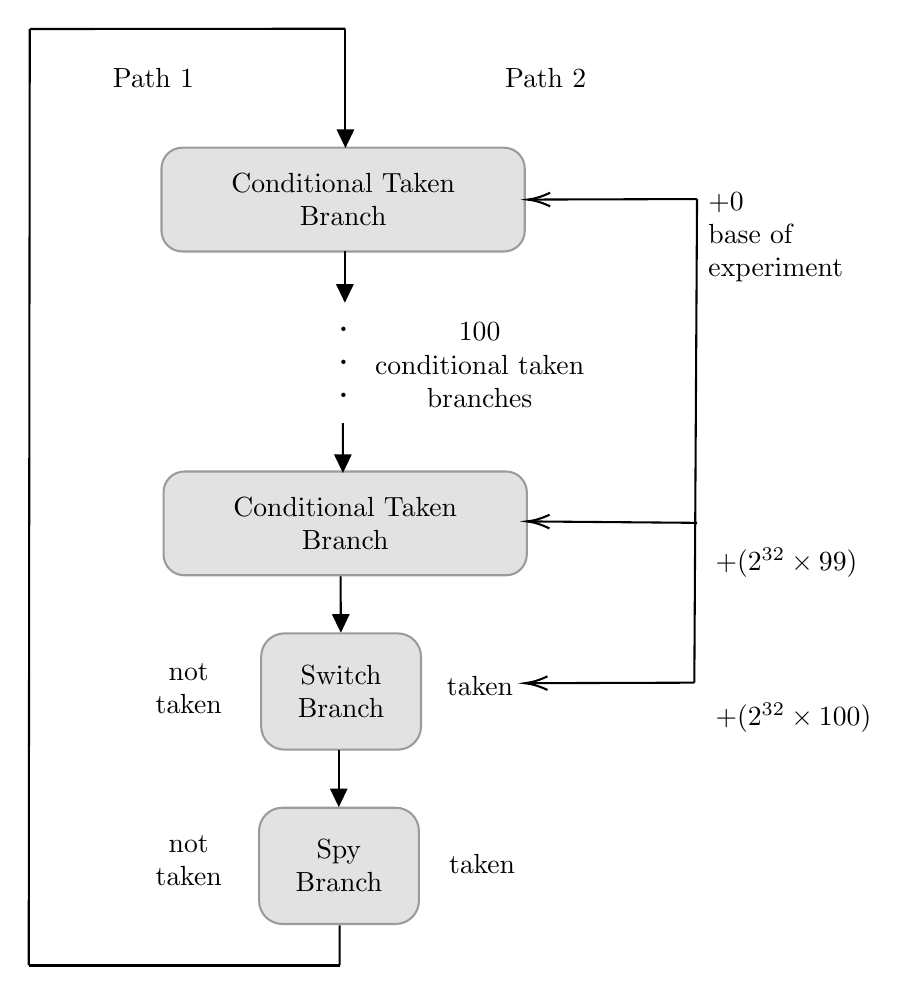
\begin{tikzpicture}[x=0.75pt,y=0.75pt,yscale=-1,xscale=1]

\draw  [color={rgb, 255:red, 155; green, 155; blue, 155 }  ,draw opacity=1 ][fill={rgb, 255:red, 226; green, 226; blue, 226 }  ,fill opacity=1 ] (237,579.2) .. controls (237,573.01) and (242.01,568) .. (248.2,568) -- (302.8,568) .. controls (308.99,568) and (314,573.01) .. (314,579.2) -- (314,612.8) .. controls (314,618.99) and (308.99,624) .. (302.8,624) -- (248.2,624) .. controls (242.01,624) and (237,618.99) .. (237,612.8) -- cycle ;
\draw    (276.22,446) -- (276.37,480.69) ;
\draw [shift={(276.39,483.69)}, rotate = 269.75] [fill={rgb, 255:red, 0; green, 0; blue, 0 }  ][line width=0.08]  [draw opacity=0] (8.93,-4.29) -- (0,0) -- (8.93,4.29) -- cycle    ;
\draw  [color={rgb, 255:red, 155; green, 155; blue, 155 }  ,draw opacity=1 ][fill={rgb, 255:red, 226; green, 226; blue, 226 }  ,fill opacity=1 ] (190.97,416) .. controls (190.97,410.48) and (195.44,406) .. (200.97,406) -- (355.97,406) .. controls (361.49,406) and (365.97,410.48) .. (365.97,416) -- (365.97,446) .. controls (365.97,451.52) and (361.49,456) .. (355.97,456) -- (200.97,456) .. controls (195.44,456) and (190.97,451.52) .. (190.97,446) -- cycle ;
\draw  [color={rgb, 255:red, 155; green, 155; blue, 155 }  ,draw opacity=1 ][fill={rgb, 255:red, 226; green, 226; blue, 226 }  ,fill opacity=1 ] (238,495.2) .. controls (238,489.01) and (243.01,484) .. (249.2,484) -- (303.8,484) .. controls (309.99,484) and (315,489.01) .. (315,495.2) -- (315,528.8) .. controls (315,534.99) and (309.99,540) .. (303.8,540) -- (249.2,540) .. controls (243.01,540) and (238,534.99) .. (238,528.8) -- cycle ;
\draw  [color={rgb, 255:red, 155; green, 155; blue, 155 }  ,draw opacity=1 ][fill={rgb, 255:red, 226; green, 226; blue, 226 }  ,fill opacity=1 ] (189.97,260) .. controls (189.97,254.48) and (194.44,250) .. (199.97,250) -- (355,250) .. controls (360.52,250) and (365,254.48) .. (365,260) -- (365,290) .. controls (365,295.52) and (360.52,300) .. (355,300) -- (199.97,300) .. controls (194.44,300) and (189.97,295.52) .. (189.97,290) -- cycle ;
\draw    (448,274.74) -- (368.31,274.99) ;
\draw [shift={(366.31,275)}, rotate = 359.82] [color={rgb, 255:red, 0; green, 0; blue, 0 }  ][line width=0.75]    (10.93,-3.29) .. controls (6.95,-1.4) and (3.31,-0.3) .. (0,0) .. controls (3.31,0.3) and (6.95,1.4) .. (10.93,3.29)   ;
\draw    (448,430.74) -- (367.97,430.06) ;
\draw [shift={(365.97,430.04)}, rotate = 0.49] [color={rgb, 255:red, 0; green, 0; blue, 0 }  ][line width=0.75]    (10.93,-3.29) .. controls (6.95,-1.4) and (3.31,-0.3) .. (0,0) .. controls (3.31,0.3) and (6.95,1.4) .. (10.93,3.29)   ;
\draw    (446.69,507.74) -- (367,507.99) ;
\draw [shift={(365,508)}, rotate = 359.82] [color={rgb, 255:red, 0; green, 0; blue, 0 }  ][line width=0.75]    (10.93,-3.29) .. controls (6.95,-1.4) and (3.31,-0.3) .. (0,0) .. controls (3.31,0.3) and (6.95,1.4) .. (10.93,3.29)   ;
\draw    (448,274.74) -- (446.69,507.74) ;
\draw    (126,644) -- (275.79,644) ;
\draw    (275.77,624.64) -- (275.79,644) ;

\draw    (278.6,192.67) -- (278.6,247.13) ;
\draw [shift={(278.6,250.13)}, rotate = 270] [fill={rgb, 255:red, 0; green, 0; blue, 0 }  ][line width=0.08]  [draw opacity=0] (8.93,-4.29) -- (0,0) -- (8.93,4.29) -- cycle    ;
\draw    (278.6,192.67) -- (126.51,192.82) ;

\draw    (126.51,192.82) -- (126,644) ;
\draw    (275.39,540.3) -- (275.39,564.69) ;
\draw [shift={(275.39,567.69)}, rotate = 270] [fill={rgb, 255:red, 0; green, 0; blue, 0 }  ][line width=0.08]  [draw opacity=0] (8.93,-4.29) -- (0,0) -- (8.93,4.29) -- cycle    ;
\draw    (277.33,382.67) -- (277.38,403.69) ;
\draw [shift={(277.39,406.69)}, rotate = 269.87] [fill={rgb, 255:red, 0; green, 0; blue, 0 }  ][line width=0.08]  [draw opacity=0] (8.93,-4.29) -- (0,0) -- (8.93,4.29) -- cycle    ;
\draw    (278.33,300) -- (278.33,321.67) ;
\draw [shift={(278.33,324.67)}, rotate = 270] [fill={rgb, 255:red, 0; green, 0; blue, 0 }  ][line width=0.08]  [draw opacity=0] (8.93,-4.29) -- (0,0) -- (8.93,4.29) -- cycle    ;

\draw (165,210) node [anchor=north west][inner sep=0.75pt]   [align=left] {\textbf{{\fontfamily{helvet}\selectfont Path 1}}};
\draw (354,210) node [anchor=north west][inner sep=0.75pt]   [align=left] {\textbf{{\fontfamily{helvet}\selectfont Path 2}}};
\draw (182,580) node [anchor=north west][inner sep=0.75pt]   [align=left] {\begin{minipage}[lt]{29.37pt}\setlength\topsep{0pt}
\begin{center}
\textbf{{\fontfamily{helvet}\selectfont not}}\\\textbf{{\fontfamily{helvet}\selectfont taken}}
\end{center}

\end{minipage}};
\draw (327,589) node [anchor=north west][inner sep=0.75pt]   [align=left] {\textbf{{\fontfamily{helvet}\selectfont taken}}};
\draw (275.5,596) node   [align=left] {\begin{minipage}[lt]{37.87pt}\setlength\topsep{0pt}
\begin{center}
\textbf{{\fontfamily{helvet}\selectfont Spy }}\\\textbf{{\fontfamily{helvet}\selectfont Branch}}
\end{center}

\end{minipage}};
\draw (277.48,275) node   [align=left] {\begin{minipage}[lt]{90.38pt}\setlength\topsep{0pt}
\begin{center}
\textbf{{\fontfamily{helvet}\selectfont Conditional Taken}}\\\textbf{{\fontfamily{helvet}\selectfont Branch}}
\end{center}

\end{minipage}};
\draw (452,270) node [anchor=north west][inner sep=0.75pt]   [align=left] {\textbf{{\fontfamily{helvet}\selectfont $+0$}}\\\textbf{{\fontfamily{helvet}\selectfont base of }}\\\textbf{{\fontfamily{helvet}\selectfont experiment}}};
\draw (452,437.69) node   [anchor=north west][align=left] {\textbf{{\fontfamily{helvet}\selectfont $+(2^{32} \times 99)$}}};
\draw (452,512.69) node   [anchor=north west][align=left] {\textbf{{\fontfamily{helvet}\selectfont $+(2^{32} \times 100)$}}};
\draw (284,333) node [anchor=north west][inner sep=0.75pt]   [align=left] {\begin{minipage}[lt]{86.6pt}\setlength\topsep{0pt}
\begin{center}
\textbf{{\fontfamily{helvet}\selectfont 100}}\\\textbf{{\fontfamily{helvet}\selectfont conditional taken}}\\\textbf{{\fontfamily{helvet}\selectfont branches}}
\end{center}

\end{minipage}};
\draw (278.47,431) node   [align=left] {\begin{minipage}[lt]{90.38pt}\setlength\topsep{0pt}
\begin{center}
\textbf{{\fontfamily{helvet}\selectfont Conditional Taken}}\\\textbf{{\fontfamily{helvet}\selectfont Branch}}
\end{center}

\end{minipage}};
\draw (274,335) node [anchor=north west][inner sep=0.75pt]   [align=left] {\textbf{.}\\\textbf{.}\\\textbf{.}};
\draw (182,497) node [anchor=north west][inner sep=0.75pt]   [align=left] {\begin{minipage}[lt]{29.37pt}\setlength\topsep{0pt}
\begin{center}
\textbf{{\fontfamily{helvet}\selectfont not}}\\\textbf{{\fontfamily{helvet}\selectfont taken}}
\end{center}

\end{minipage}};
\draw (326,503.2) node [anchor=north west][inner sep=0.75pt]   [align=left] {\textbf{{\fontfamily{helvet}\selectfont taken}}};
\draw (276.5,512) node   [align=left] {\begin{minipage}[lt]{38.43pt}\setlength\topsep{0pt}
\begin{center}
\textbf{{\fontfamily{helvet}\selectfont Switch }}\\\textbf{{\fontfamily{helvet}\selectfont Branch}}
\end{center}

\end{minipage}};


\end{tikzpicture}
